%!TEX root = ../main.tex
\section{Thuật toán đề xuất}

\begin{frame}{Cơ chế chọn tác vụ hỗ trợ - MAB}
    \begin{alertblock}{Mô hình hóa việc chọn tác vụ để lai ghép bằng MAB}
        \begin{mydef}[Lựa chọn]
            Với mỗi tác vụ $T_k$, sẽ có $K-1$ lựa chọn, tương ứng với $K-1$ tác vụ $T_{k'}$ mà $k' \in \{1, \ldots, K\} \text{ và } k' \ne k$.
            \label{def:propose:action}
        \end{mydef}

        \begin{mydef}[Phần thưởng]
            Sau khi tác vụ $T_{k'}$ được lựa chọn để ghép cặp với tác vụ $T_{k}$, phần thưởng của việc chọn tác vụ $T_{k'}$ được định nghĩa như sau:
            \begin{equation}
                r(k, k') = \left\{
                    \begin{array}{ll}
                        1 \text{ nếu } f_k(c) < f_k(p) , \exists p \in P^k \\\
                        0 \text{ trong các trường hợp khác}.
                    \end{array}
                  \right.
            \end{equation}
            \begin{itemize}
                \item $c$ là con sinh ra trong quá trình lai ghép khác tác vụ
                \item $f_k(.)$ là hàm đánh giá của tác vụ $T_k$
            \end{itemize}
            \label{def:propose:reward}
        \end{mydef}
    \end{alertblock}
\end{frame}

\begin{frame}{Cách giải bài toán con chọn tác vụ hỗ trợ - KLUCB}
    \begin{block}{Giả định}
        \begin{itemize}
            \item \textbf{Phần thưởng}: Biến ngẫu nhiên với giá trị $\{0, 1\}$
            \item \textbf{Giả định}: Phần thưởng sinh từ phân phối Bernoulli chưa biết trước.
        \end{itemize}
    \end{block}
    \begin{block}{Cách giải - KLUCB}
        \begin{equation}
            k' = \underset{j}{\text{argmax }} \mu(j) + \frac{1 + t \times log^2(t) }{N(j)}
            \label{eq:propose:klucb}
        \end{equation}
        \begin{itemize}
            \item $\mu(j)$ là giá trị trung bình ước lượng được của phần thưởng khi lựa chọn $j$
            \item $N(j)$ là tổng số lần thuật toán đã lựa chọn $j$
            \item $t$ là tổng số của tất cả các lần lựa chọn
        \end{itemize}
    \end{block}
    \begin{block}{Tham khảo lý thuyết tại}
        \fullcite{lattimore2020bandit}
    \end{block}
\end{frame}

\begin{frame}{Khung giải thuật đề xuất - Ma2BEA}
    \begin{algorithm}[H]
        \caption{\gls{propose} trong mỗi thế hệ của tác vụ $T_k$}
        \fontsize{6pt}{10}\selectfont
        \begin{algorithmic}[1]
            \State Khởi tạo quần thể con $P_{(c)}^k=\emptyset$
            \While{số con sinh ra $< N$}
                \State Chọn ngẫu nhiên cá thể cha $p_a$ từ $P^k$
                \If{$rand(0, 1) < rmp$}
                    \State {\color{red} Chọn tác vụ $T_{k'}$ sử dụng phương trình \gls{klucb} trong Công thức \ref{eq:propose:klucb}}
                    \State Chọn ngẫu nhiên cá thể mẹ $p_b$ từ $P^{k'}$
                    \State $c = $ \emph{Lai ghép khác tác vụ} giữa $p_a$ và $p_b$
                \Else
                    \State Chọn ngẫu nhiên cá thể mẹ $p_b$ từ $P^k$
                    \State $c = $ \emph{Lai ghép cùng tác vụ} giữa $p_a$ và $p_b$
                \EndIf
                \State $c =$ Đột biến $c$
                \State Đánh giá cá thể con $c$
                \State {\color{red} Cập nhật lại ước lượng $\mu(k')$ và số lượng $N(k')$ cho \gls{klucb} nếu $c$ được sinh ra từ việc \emph{Lai ghép khác tác vụ}}
                \State $P^k_{(c)} = P^k_{(c)} \cup \{c\}$
            \EndWhile
            \State $P^k \leftarrow$ Chọn $N$ cá thể tốt nhất từ $P^k \cup P^k_{(c)}$ để tạo lại $P^k$ cho thế hệ tiếp theo
        \end{algorithmic}
        \label{alg:propose:generation}
    \end{algorithm}
\end{frame}

\begin{frame}{Cấu trúc cập nhật tuần tự - 1}
    \begin{algorithm}[H]
        \caption{Giả mã của toàn bộ \gls{propose}}
        \begin{algorithmic}[1]
            \For{$k \in \{1, \ldots, K\}$}
                \State Khởi tạo ngẫu nhiên $N \sim \mathbb{R}^{D_{unified}}$ cá thể để tạo ra quần thể $P^k$
                \State Đánh giá $P^k$ trên $f_k$
            \EndFor
            \While{điều kiện kết thúc chưa thỏa mãn}
                \For{$k \in $ hoán vị ngẫu nhiên của $({1, \ldots, K})$}
                    \State Thực hiện Thuật toán \ref{alg:propose:generation} cho tác vụ $T_k$
                \EndFor
            \EndWhile
        \end{algorithmic}
        \label{alg:propose:propose}
    \end{algorithm}
\end{frame}

\begin{frame}{Cấu trúc cập nhật tuần tự - 2}
    \begin{block}{Ví dụ cho tác dụng của cập nhật tuần tự trong \gls{propose}}
        \begin{figure}
            \centering
            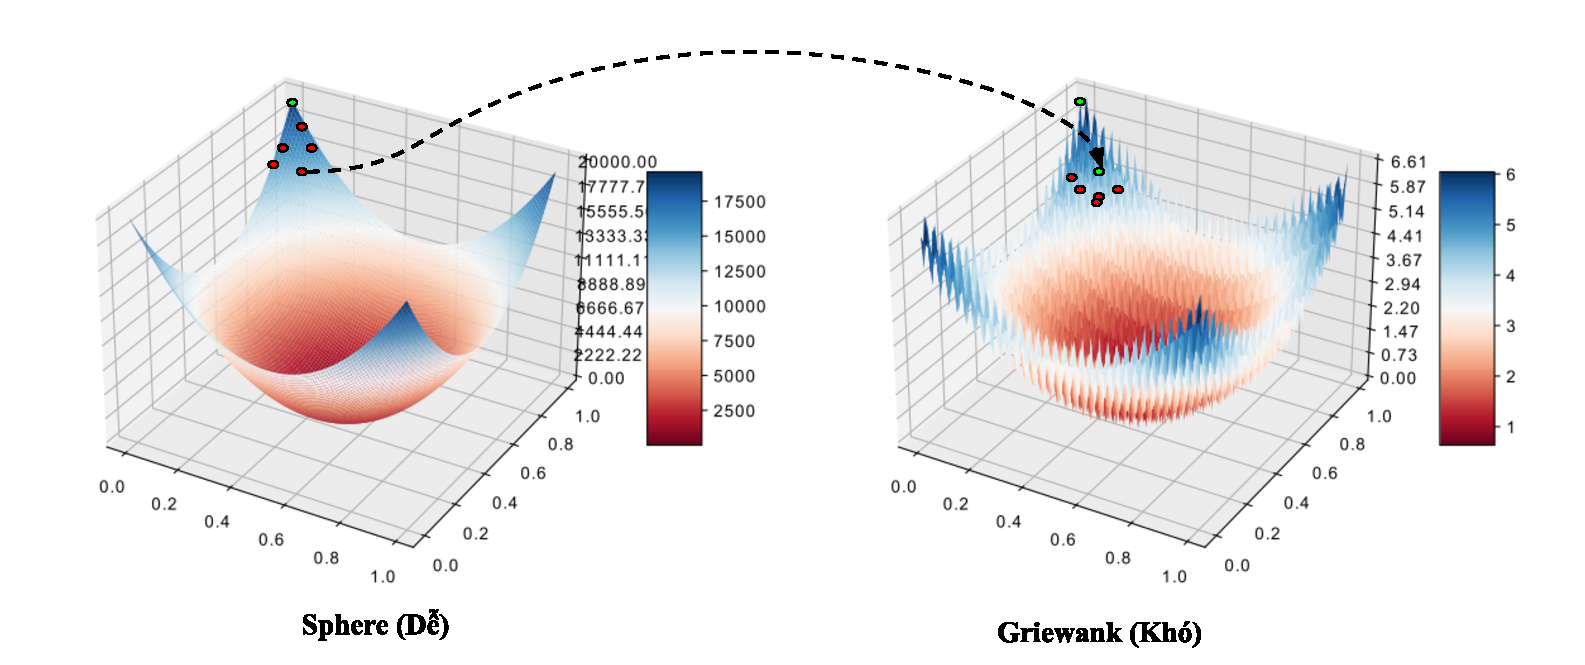
\includegraphics[width=\linewidth]{figure/propose/sequential-motivation.eps}
            \caption{Cập nhật tuần tự trên hai tác vụ có địa hình hàm mục tiêu tương đồng. Trục tung, trục hoành là giá trị của nghiệm. Trục thẳng đứng là giá trị hàm mục tiêu.}
            \label{fig:propsoe:sequential-motivation}
        \end{figure}
    \end{block}
\end{frame}

\begin{frame}{Tóm tắt đóng góp}
    \begin{columns}
        \begin{column}{0.48\textwidth}
            \begin{block}{Các đề xuất tại \gls{propose}}
                \begin{itemize}
                    \item Mô hình hóa ghép cặp trao đổi tri thức giữa các tác vụ trên mô hình MAB, giải bằng KLUCB.
                    \item Thay cấu trúc của MFEA bằng cấu trúc trao đổi tuần tự.
                \end{itemize}
            \end{block}
            \begin{block}{So với MFEA}
                \begin{itemize}
                    \item SBSGA, MaTGA, \gls{propose} đều trội hơn ở cơ chế trao đổi tri thức tự thích ứng.
                \end{itemize}
            \end{block}
        \end{column}
        \begin{column}{0.48\textwidth}
            \begin{block}{So với MaTGA}
                \begin{itemize}
                    \item \gls{propose} nhanh hơn, vì chỉ phân tích dữ liệu hàm mục tiêu ($\sim \mathbb{R}^{N \times K}$), thay vì phân tích dữ liệu lịch sử quần thể ($\sim \mathbb{R}^{D_{unified} \times N \times K}$).
                    \item Không phụ thuộc biểu diễn quần thể.
                    \item \gls{propose} ít tham số hơn, không cần chọn lưu lại quá khứ bao nhiêu cá thể như MaTGA.
                \end{itemize}
            \end{block}
            \begin{block}{So với SBSGA}
                \begin{itemize}
                    \item Cách ghép cặp của \gls{propose} có nên tảng lý thuyết hơn so với SBSGA
                \end{itemize}
            \end{block}        
        \end{column}
    \end{columns}
\end{frame}

\begin{frame}{Áp dụng - Tối ưu nhiều mạng nơ-ron}
    \begin{columns}
        \begin{column}{0.48\textwidth}
            \begin{block}{Bài toán học tăng cường}
                \begin{figure}
                    \centering
                    \includegraphics[width=0.7\linewidth]{figure/propose/mdp.png}
                    \caption{Tương tác giữa tác tử (Agent) và môi trường (Environment) trong mô hình Markov Decision Process.}
                    \label{fig:propose:mdp}
                \end{figure}
            \end{block}
        \end{column}
        \begin{column}{0.48\textwidth}
            \begin{block}{Lý do áp dụng tiến hóa đa nhiệm cho học tăng cường}
                \begin{itemize}
                    \item Hàm mục tiêu không có gradient.
                    \item Có nhiều môi trường tương tự nhau, việc giải cùng nhau hy vọng sẽ cho kết quả tối ưu hơn.
                \end{itemize}
            \end{block}
        \end{column}
    \end{columns}
    \begin{alertblock}{Giải nhiều bài toán học tăng cường}
        \textbf{Cho:} $K$ môi trường $\{E_1, \ldots, E_K\}$
        \begin{columns}
            \begin{column}{0.48\textwidth}
                \begin{equation}
                    \underset{\theta_k}{\text{maximize }} F(\theta_k; E_k) = \sum_{t=1}^{T} r_t
                \end{equation}
            \end{column}
            \begin{column}{0.48\textwidth}
                \begin{itemize}
                    \item $\theta_k$: tham số mô hình đưa quyết định (mạng nơ ron) 
                    \item $r_t$: phần thưởng tại thời điểm $t$
                \end{itemize}
            \end{column}
        \end{columns}
    \end{alertblock}
\end{frame}

